
\documentclass[aspectratio=169]{beamer}
\usetheme{Boadilla}

\usepackage{qrcode}

\usepackage[utf8]{inputenc}       % Codificação de entrada
\usepackage[T1]{fontenc}          % Codificação de saída
\usepackage[portuguese]{babel}   % Idioma
\usepackage{XCharter}             % Fonte principal
\AtBeginDocument{\fontsize{12}{12}\selectfont}

%\usepackage{geometry}
%\geometry{papersize={210mm,150mm}}
\usepackage{tikz}
\usepackage{pgf-pie} % necessário para gráficos de pizza

\usepackage{color}
\usepackage{graphicx}
\usepackage{amsmath, amssymb, amsfonts}
\usepackage{bm}
\usepackage{booktabs}
\usepackage{multirow}
\usepackage{caption}
\usepackage{subfigure}
\usepackage{wrapfig}
\usepackage{multicol}
\usepackage{sidecap}
\usepackage{tikz}
\usepackage{listings}
\usepackage{siunitx}
\usepackage{pdfpages}
\usepackage{float}
\usepackage{hyperref}
\usepackage{academicons}
\usepackage{setspace}

\newcommand{\eng}[1]{\textsl{#1}}
\newcommand{\cod}[1]{\texttt{#1}}

\usepackage{tikz}
\usetikzlibrary{shapes.geometric, arrows, positioning}

% Definição de estilos para o fluxograma
\tikzstyle{startstop} = [ellipse, rounded corners, minimum width=2cm, minimum height=0.8cm, text centered, draw=black, fill=gray!20]
\tikzstyle{process} = [rectangle, minimum width=3.5cm, minimum height=1cm, text width=4.5cm, text centered, draw=black, fill=white]
\tikzstyle{decision} = [diamond, aspect=2, minimum width=3cm, minimum height=1cm, text centered, draw=black, fill=white]
\tikzstyle{arrow} = [thick,->,>=stealth]

% Definição de cores profissionais
\definecolor{mipsblue}{RGB}{50, 90, 120}
\definecolor{mipsred}{RGB}{150, 30, 30}

\title[Arquitetura de Computadores]{\huge  Experimento 2} %note that the optional arg in '[]' are displayed in the left column throughout the complete presentation
% adapt accordingly
% e.g., M.Sc. Intermediate Thesis Report
% or     B.Sc. Intermediate Thesis Report


\author[Prof. Dr. Oscar Eduardo Anacona Mosquera]{Prof. Dr. Oscar Eduardo Anacona Mosquera \newline\newline 
	\scriptsize{oscar.mosquera@ufmt.br}
}%note that the optional arg in '[]' are displayed in the left column throughout the complete presentation



\AtBeginSection[]
{
	\begin{frame}{Sumário}
		\tableofcontents[currentsection]
	\end{frame}
}


\begin{document}

	\begin{frame}[plain]
		\titlepage
	\end{frame}
	
	\begin{frame}{Sumário}
		\tableofcontents
	\end{frame}
	
%=======================================================================================
%\section{Introdução}
%=======================================================================================

% --- SLIDE: NOVO PROJETO ---
\begin{frame}{Passo 1: Novo Projeto para Análise de Dados}
	\begin{itemize}
		\item Crie um novo projeto no Quartus: \textit{File $\rightarrow$ New Project Wizard}.
		\item Nome do projeto: \textbf{Sistemas\_Numericos}.
		\item Crie um novo arquivo VHDL (\textit{File $\rightarrow$ New $\rightarrow$ VHDL File}).
	\end{itemize}
	\begin{block}{Objetivo}
		Observar como o ModelSim interpreta o mesmo conjunto de bits (32 bits) de formas diferentes (Sinalizado, Sem Sinal, Float).
	\end{block}
	%\begin{figure}
	%\includegraphics[width=0.5\textwidth]{novo_projeto_quartus.png}
	%\caption{Configuração inicial do projeto.}
	%\end{figure}
\end{frame}

% --- SLIDE: CODIGO VHDL ---
\begin{frame}[fragile]{Passo 2: Entidade sem Saídas}
	\justifying
	Criaremos uma entidade com duas entradas de 32 bits. Não precisamos de saídas, pois observaremos os sinais internamente no ModelSim.
	
	\begin{lstlisting}[language=VHDL, basicstyle=\tiny]
		library ieee;
		use ieee.std_logic_1164.all;
		
		entity Sistemas_Numericos is
		port (
		dado_A : in std_logic_vector(31 downto 0);
		dado_B : in std_logic_vector(31 downto 0)
		);
		end entity;
		
		architecture rtl of Sistemas_Numericos is
		begin
		-- Apenas para evitar otimizacoes do compilador
		end architecture;
	\end{lstlisting}
\end{frame}

% --- SLIDE: TESTBENCH DE DADOS ---
\begin{frame}[fragile]{Passo 3: Testbench com Valores Estratégicos}
	\justifying
	No Testbench, vamos injetar valores hexadecimais que mudam drasticamente de sentido dependendo do \textit{Radix}.
	
	%\begin{lstlisting}[language=VHDL, basicstyle=\tiny]
	%-- No processo de estimulos do Testbench
	%-- Exemplo: Valor que representa 12.5 em Float IEEE-754
	%dado_A <= x"41480000"; 
	%
	%-- Exemplo: Valor que parece negativo em Signed
	%dado_B <= x"FFFFFFFF"; 
	%
	%wait for 100 ns;
	%
	%dado_A <= x"C1480000"; -- -12.5 em Float
	%dado_B <= x"0000000A"; -- 10 em Decimal
	%\end{lstlisting}
	\begin{figure}
		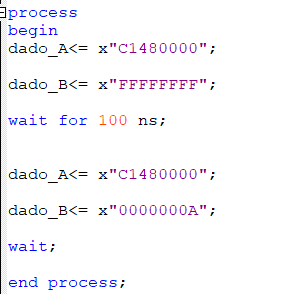
\includegraphics[width=0.3 \textwidth]{Figs/tut_fig20.png}
	\end{figure}
\end{frame}

% --- SLIDE: MODELSIM RADIX ---
\begin{frame}{Passo 4: Radix no ModelSim}
	\justifying
	Após carregar a simulação no ModelSim:
	\begin{enumerate}
		\item Selecione o sinal na janela \textbf{Wave}.
		\item Clique com o botão \textbf{Direito}.
		\item Vá em \textbf{Radix} e experimente as opções:
		\begin{itemize}
			\item \textbf{Unsigned}: Para valores naturais (0 a $2^{32}-1$).
			\item \textbf{Decimal}: Para valores sinalizados (Complemento de 2).
			\item \textbf{Hexadecimal}: Padrão de bits.
			\item \textbf{Floating Point $\rightarrow$ 32-bit}: Para ver o valor real (IEEE-754).
		\end{itemize}
	\end{enumerate}
	% \begin{figure}
		%\includegraphics[width=0.6\textwidth]{modelsim_radix_menu.png}
		%\caption{Menu de alteração de representação numérica.}
		%\end{figure}
	\end{frame}
	
	% --- SLIDE: COMPARACAO ---
	\begin{frame}{Passo 5: Analisando os Resultados}
		\justifying
		Observe como o valor \texttt{x"FFFFFFFF"} se transforma:
		\begin{itemize}
			\item Em \textbf{Unsigned}: 4.294.967.295
			\item Em \textbf{Decimal (Signed)}: -1
		\end{itemize}
		
		Observe o valor \texttt{x"41480000"}:
		\begin{itemize}
			\item Em \textbf{Hex}: 41480000
			\item Em \textbf{Float 32-bit}: 12.5
		\end{itemize}
		
		\begin{block}{Conclusão}
			O hardware não sabe o que é um "número", ele apenas processa bits. É o projetista quem define a interpretação através da lógica e da visualização.
		\end{block}
		%\begin{figure}
		%\includegraphics[width=0.7\textwidth]{resultado_comparativo_wave.png}
		%\end{figure}
	\end{frame}






\end{document}
